% The section about the usage of the given MARS-Framework
% @author Kalvin Döge
%


\section{Anbindung an das MARS-Framework}\label{sec:mars-connection}

Die Anbindung zum MARS-Framework geschieht bei den im technischen Modell erläuterten Klassen durch Fassaden.
Im Folgen wird näher erläutert, welche Fassaden durch welche Klasse implementiert werden und wie sie damit in die Simulationsumgebung vom MARS-Framework eingebunden werden:

\begin{figure}[h]
    \centering
    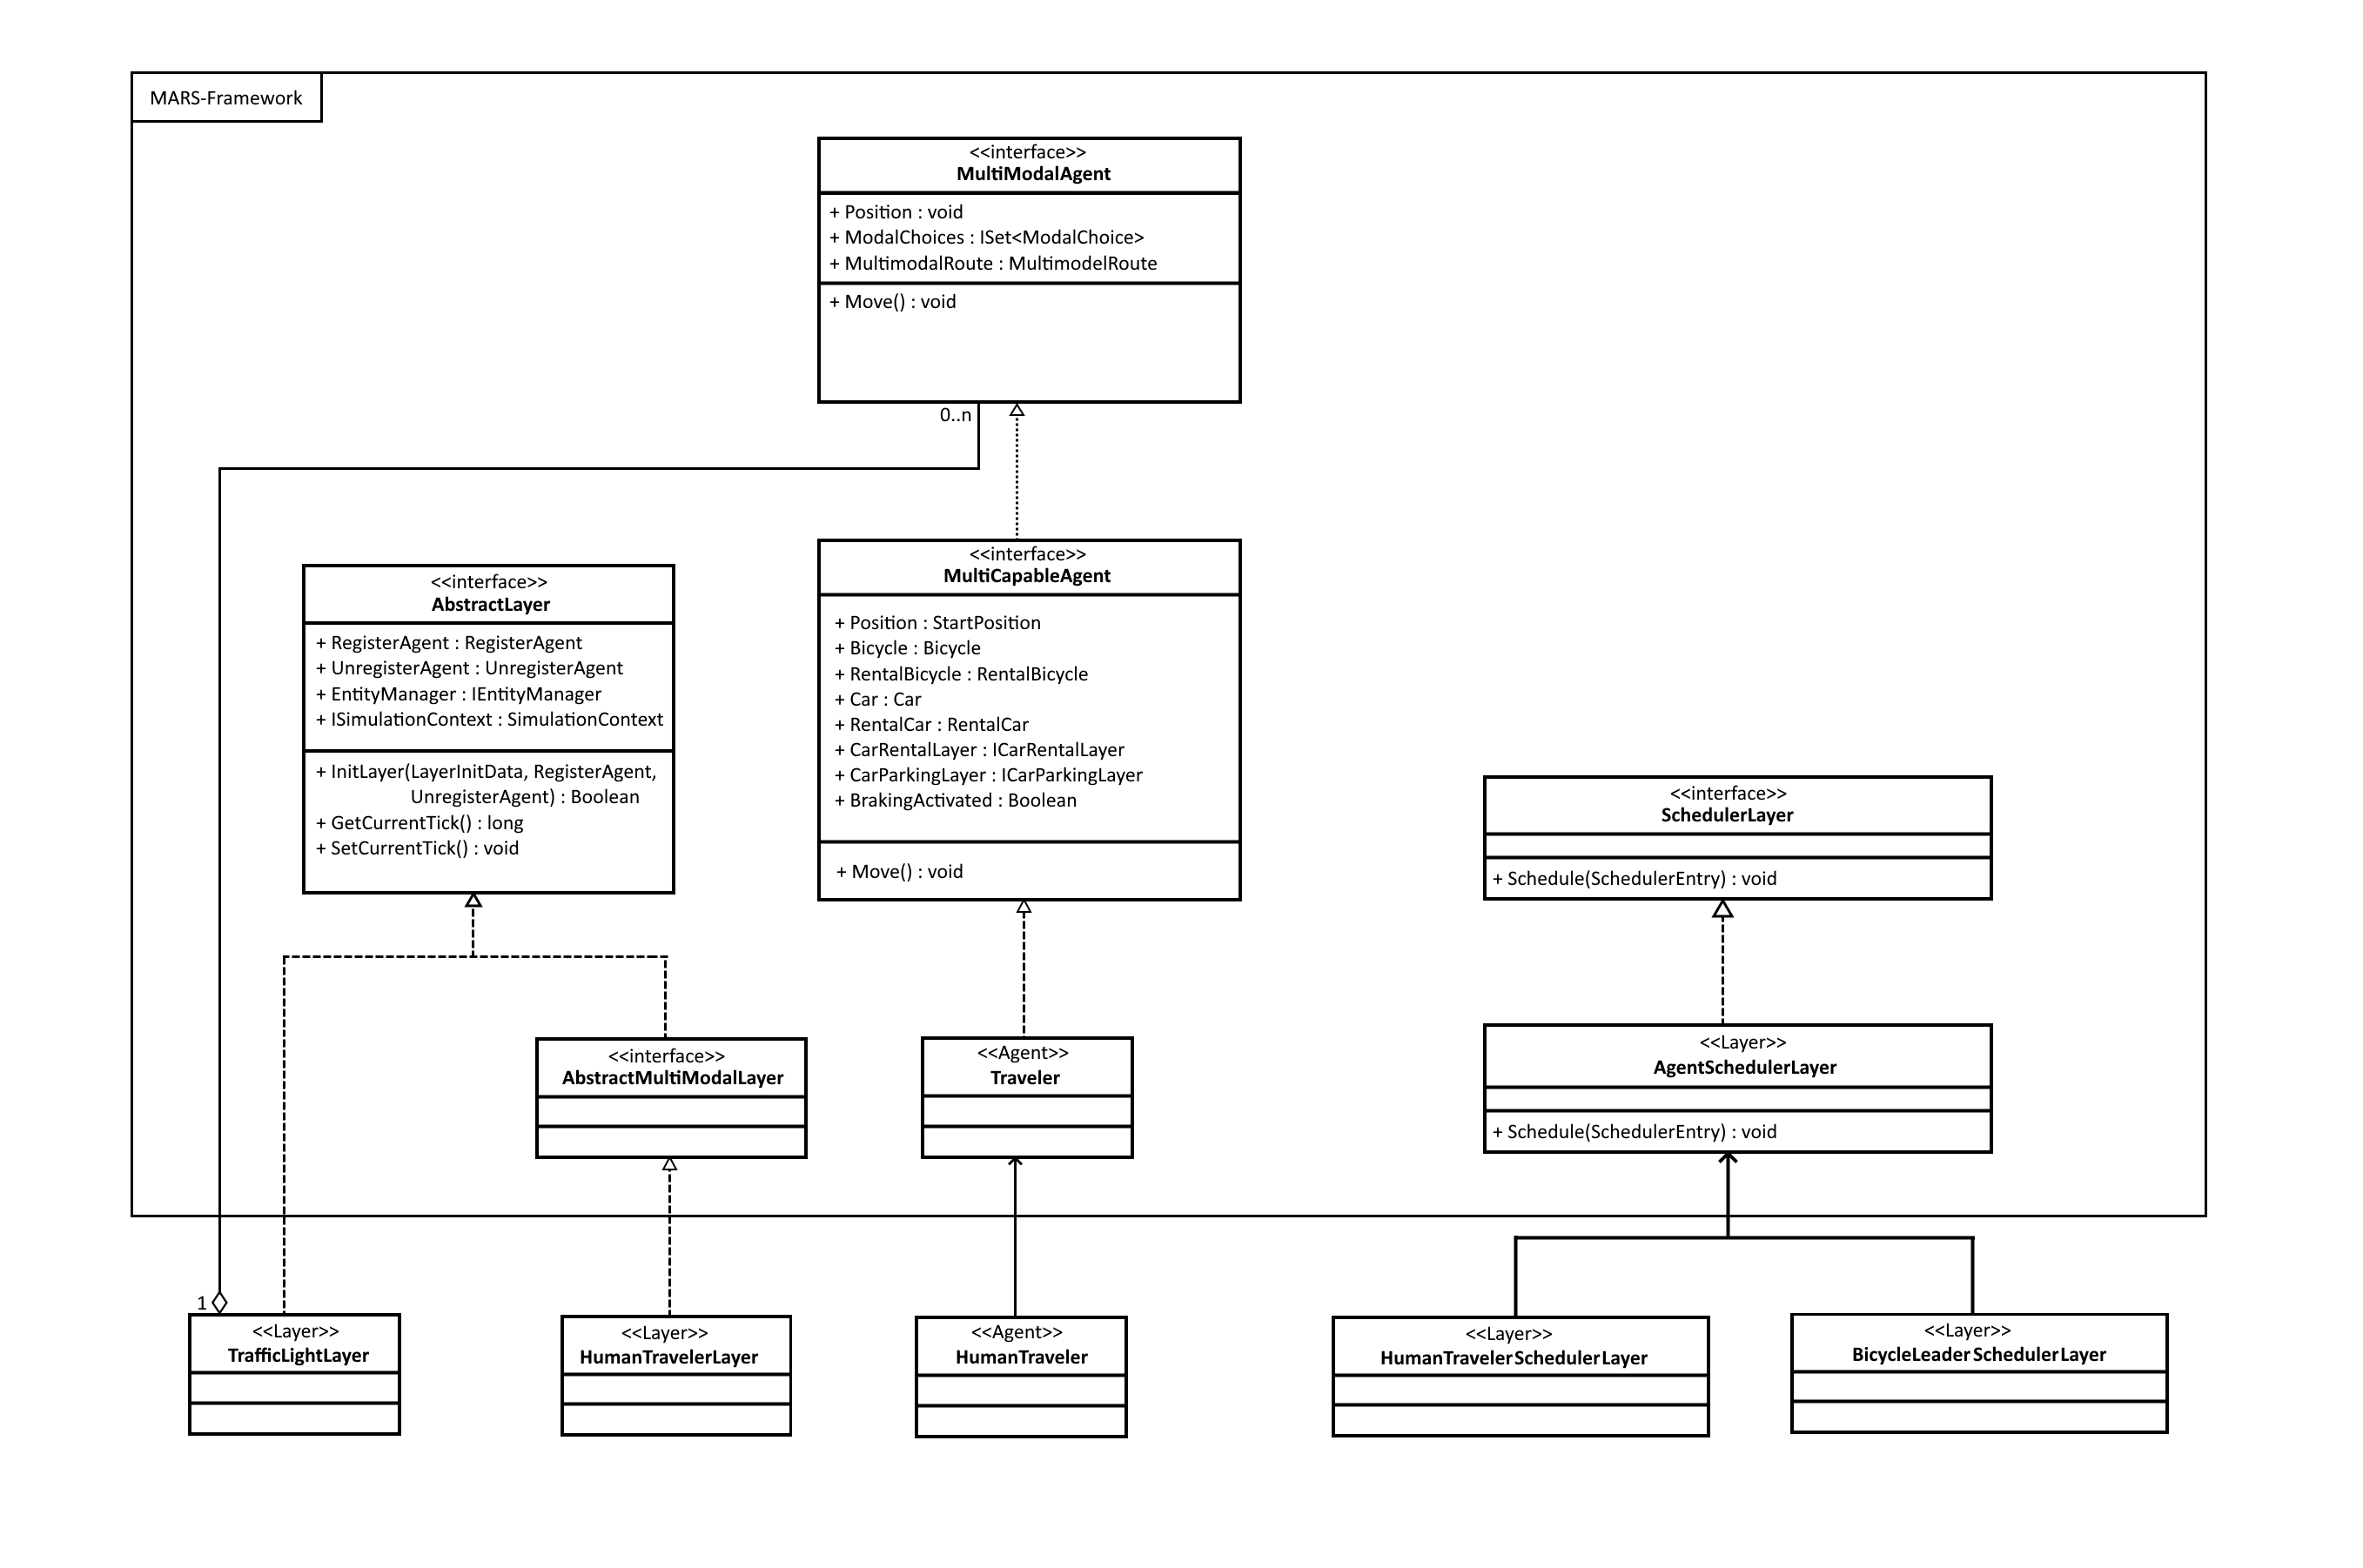
\includegraphics[width=1.00\textwidth]{mars-connection-diagramm}~\caption{Die Anbindung an bestehenden Fassaden des MARS-Frameworks}
    \label{fig:mars-connection}
\end{figure}

Auch sind hier in dem technischen Datenmodell~\ref{fig:mars-connection} wieder der Übersichtlich- und Lesbarkeit halber überflüssige Fassaden, Eigenschaften und Funktionen weggelassen worden.

\textbf{Layer \code{TrafficLightLayer} und \code{HumanTravelerLayer}:}
\begin{itemize}
    \item Der \code{TrafficLightLayer} und \code{HumanTravelerLayer} implementieren den \code{AbstractLayer} und erhalten dadurch Zugriff auf den \code{RegisterAgent},\code{UnregisterAgent} und \code{EntityManager}, mit dem die Layer selbstständig der Simulation Entitäten und Agenten hinzufügen oder nehmen können.
    \item Durch das Initialisieren über die \code{Init(...)}-Funktion und dem \code{SimulationContext}, können beide \code{Layer} über die Konfiguration festgelegten Eingabedaten erhalten und alle \code{TrafficLight}s oder \code{HumanTraveler} erstellen.
    \item Mit den Funktionen \code{GetCurrentTick()} und \code{SetCurrentTick()} lässt sich auch der derzeitige Simulationszeitpunkt feststellen, sowie die \code{Tick()}-Methode ausführen beim Setzen eines neuen Simulationsschrittwertes.
    \item Der \code{MultiModalAgent} benötigt eine Referenz auf den \code{TrafficLightLayer}, da alle erbenden Klassen auf diesen \code{Layer} zugreifen müssen. \code{MultiModalAgent} ist dabei die einzige Klasse, die über die Annotation \code{[PropertyDescription]} eine Instanz des \code{TrafficLightLayers} und nicht einen \code{Null}-Wert gesetzt bekommt.
\end{itemize}

\textbf{Agent \code{HumanTraveler}}
\begin{itemize}
    \item Der \code{HumanTraveler} implementiert den \code{Traveler}, der aber über keine weiteren für diese Simulation relevanten Eigenschaften oder Funktionen verfügt.
    \item Zudem implementiert er den \code{MultiCapableAgent}, der für jede Modalität eine Eigenschaft besitzt und den dazugehörigen \code{Layer}.
    \item Die Referenz auf diese Modalitäten wird an die Unterklassen weitergeben, zum Beispiel den \code{BicycleLeader}, die mit der \code{Move()}-Funktion dann die Bewegung auf dem \code{ISpatialMediatorGraph} ausführen.
    \item Zuletzt implementiert \code{HumanTraveler} noch den \code{MultiModalAgent}, der mit der \code{Position} jedem Agenten seinen Standort in der Simulation angibt, mit \code{ModalChoices} dem Agenten die nutzbaren Modalitäten und mit \code{MultimodalRoute} die in der Simulation fahrende Route vererbt.
\end{itemize}

\textbf{Layer \code{HumanTravelerSchedulerLayer} und \code{BicycleLeaderSchedulerLayer}}
\begin{itemize}
    \item Beide \code{Layer} implementieren den \code{AgenSchedulerLayer}, der eine Standard-Implementation der \code{Schedule(SchedulerEntry)}-Funktion bereitstellt und nur zwei angegebene Argumente benötigt beim implementieren: Den zu erschaffenden \code{Agent}en und den \code{Layer}, zu dem dieser hinzugefügt werden soll.
    \item Die Fassade für den \code{AgentSchedulerLayer}, der intern die verschiedenen \code{AgentSchedulerLayer} vereint, schreibt \code{Schedule(SchedulerEntry)} zum Implementieren vor und führt dann, sobald ein Eintrag zeitlich passt, die Funktion mit dem Eintrag aus.
\end{itemize}
